\documentclass[12pt]{article}

\usepackage{sbc-template}
\usepackage{graphicx,url}
\usepackage[brazil]{babel}
\usepackage[latin1]{inputenc}
\usepackage{lscape}
\usepackage{geometry}
\usepackage{float}
\usepackage{algorithm2e}
\usepackage{multicol}
\usepackage{amsmath}
\usepackage{amsfonts}
\usepackage{amssymb}
\usepackage{makeidx}
\usepackage{graphicx}
\usepackage{lmodern}
\usepackage{enumerate}
\usepackage{latexsym}
\usepackage{longtable}
\usepackage[all]{xy}
\usepackage{float}
\usepackage{lscape}
\usepackage{mathrsfs}
\usepackage{fancyhdr}
\usepackage{boxedminipage}
\usepackage{enumitem}


\sloppy

\title{Algoritmo A* para resolução da Árvore Geradora de Rótulos Mínimos}

\author{Marco Cezar Moreira de Mattos\inst{1}, Rômulo Manciola Meloca\inst{1}}

\address{DACOM -- Universidade Tecnológica Federal do Paraná (UTFPR)\\
	Caixa Postal 271 -- 87301-899 -- Campo Mourão -- PR -- Brazil
	\email{\{marco.cmm,rmeloca\}@gmail.com}
}

\begin{document}

\maketitle

\begin{resumo}
	Este relatório apresenta o emprego do algoritmo A* para a resolução da Árvore Geradora de Rótulos Mínimos, tornando evidente o problema em torno deste, bem como suas origens e dificuldades e implicações. Apresenta-se os trabalhos relacionados em especial o que dá origem à implementação proposta para o problema, discutindo os resultados dos testes aplicados na solução teórica e na solução proposta.
\end{resumo}

\section{Introdução}\label{sec:introducao}

	Em teoria dos grafos há um problema muito comum: Dado um grafo $G$ não-dirigido e conexo cujas arestas $E$ sejam ponderadas e não negativas, encontrar uma árvore $T$ sobre a qual seja possível induzir um subgrafo $G'$ de $G$, tal que $G'$ seja conexo e que a soma do peso de todas as arestas $w(E')$ seja a menor possível. A este problema chama-se Problema da Árvore Geradora de Pesos Mínimos (PAGPM), do inglês \textit{Minimum Weight Spanning Tree}.

	Definindo: Um grafo $G = \{V, E\}$ é um conjunto de vértices $v \in V$ conectados por meio de arestas $E = \{\{u, v\} \mid u, v \in V \wedge u \neq v\}$; Cada aresta $e$ possui dois vértices $(u, v)$ (abuso de notação adotado), podendo esta ser omnidirecional ou bidirecional caracterizando um grafo dirigido ou não-dirigido, respectivamente. As arestas podem portar informações relativas a distâncias caracterizando um grafo cujas arestas sejam ponderadas em sua presença ou não-ponderadas na ausência destas informações; Um vértice é uma unidade mínima que porta informações que deseja-se modelar.

	Outras definições: Uma árvore $T$ não é senão um grafo bipartido, planar, acíclico e conexo, de modo que uma árvore é uma particularidade de um grafo (assim como quadrado está para retângulo); Um grafo bipartido é aquele cujos vértices podem ser divididos em dois conjuntos disjuntos, isto é, cuja interesecção entre os conjuntos seja nula; Um grafo planar é aquele que pode ser representado em um plano (bidimensional) no qual nenhuma aresta seja concorrente a qualquer outra; Um grafo acíclico é aquele que não apresenta arestas que formem um caminho que contenha um ou mais vértices repetidos; Um grafo conexo, no âmbito de grafos não-dirigidos, é aquele que conecta todos os vértices do grafo, de modo que é possível acessar qualquer vértice a partir de qualquer outro vértice.

	Mais definições: Um subgrafo $G' = \{V', E'\}$ de um grafo $G = \{V, E\}$ é um grafo em que $V' \subseteq V \wedge E' \subseteq E$; Um grafo $G'$ induzido por $V'$ é um subgrafo de $G$ em que o conjunto de arestas $E'$ é formado a partir do conjunto de vértices $V'$ tal que para todo vértice $v$ adiciona-se em $E'$ todas as arestas relacionadas a este originalmente contidas em $E$. Matematicamente define-se um grafo induzido como sendo um grafo $G' = \{V', E'\} \mid E' = \{(u, v) \in E : u, v \in V'\} \wedge V' \subseteq V \wedge E' \subseteq E$. Nota-se que também é possível induzir um grafo a partir de outros conjuntos; Uma árvore geradora $T$ é um subgrafo $G'$ de $G$ tal que este seja conexo, não-dirigido e que possua o mesmo conjunto inicial de vértices $V' = V$; Define-se o peso total das arestas $w(E')$ como sendo $\displaystyle{w(E') = \sum_{(u,v \in E')}[w(u, v)]}$.

	Para formar uma árvore geradora são necessários exatamente $|V|-1$ arestas, tal que $|V|$ seja o número de vértices pertencentes ao grafo; Esta regra advém da definição das árvores geradoras, uma vez que esta não admite ciclos e conecta todos os vértices do grafo, disto deriva-se que para conectar todos os vértices são necessárias tantas arestas quantos vértices houverem, com exceção de uma, a fim de admitir no mínimo dois vértices que sejam finais.

	Um grafo $G = \{V, E\}$, no entanto, pode admitir várias árvores geradoras. É possível discretizar o número máximo de árvores geradoras que um grafo admite fazendo a combinação do número de arestas $|E|$ em grupos de $|V|-1$, uma vez que cada árvore geradora possui $|V|-1$ arestas, isto é, $G' = \{E', V' \mid |E'| = |V|-1 \wedge V' = V\}$, conforme discutido. Fazendo a combinação matemática $\displaystyle{|E| \choose |E'|}$, obtém-se o número de conjuntos distintos que $E'$ pode assumir, gerados a partir $E$. Evidentemente, nem todas combinações possíveis são árvores geradoras à medida em que elementos do conjunto de possíveis valores para $E'$ podem admitir ciclos, descaracterizando-se como uma árvore, tampouco geradora.

	Sejam $e = |E|$ e $e' = |E'| = |V|-1$,

	\begin{center}
	$\displaystyle{C_{e}^{e'}={\frac {e!}{e'! \cdot [e-e']!}}}$
	\end{center}
	
	Nota-se que quanto mais denso for o grafo, isto é quanto maior for o número de arestas que o grafo contiver, mais árvores geradoras o grafo admite.

	Para solucionar o PAGPM é preciso obter a melhor árvore dentre todo o conjunto de árvores geradas $C = \{E'_1, E'_2, \dots, E'_n \mid n = C_{|E|,|V|-1}\}$ a qual possua o menor peso total. Obviamente o conjunto de árvores geradas para o PAGPM é grande o suficiente para que não seja viável computar todo o conjunto e buscar nele uma solução exata (em tese), ou seja, muitas soluções são até mesmo NP-Completas! O que demanda uma solução de busca inteligente. Deste modo, é possível utilizarmos busca cega, heurística ou local.

	Utilizar um algoritmo de busca implica em obter um ótimo local ao invés da solução exata, entretanto, alguns problemas de busca operam sobre um conjunto cujos elementos são linearmente independentes, de modo que o conjunto é um matroide.
	
	Análogo ao PAGPM, há ainda o Problema da Árvore Geradora de Rótulos Mínimos (PAGRM), do inglês \textit{Minimum Labelling Spanning Tree}, o que lhe difere do PAGPM é que neste, cada aresta possui um rótulo e o objetivo é encontrar um árvore geradora utilizando o menor número de rótulos possíveis. Neste caso, a combinação matemática é feita a partir do número de rótulos e não a partir do número de arestas, de modo que a computação da solução exata (não fosse a propriedade matemática explorada), levaria muito tempo para ser feita, uma vez que não sabe-se de antemão quantos rótulos distintos serão necessários para conectar todo o grafo

	Na seção que segue é demonstrado o escopo do PAGRM.	

\section{O problema}\label{sec:problema}

	Seja $G = \{V, E, L\}$ um grafo rotulado, não-dirigido e conexo, tal que $V = \{v_1, v_2 \dots v_{|V|}\}$ seja o conjunto de vértices, $E = \{(u, v) \mid u, v \in V \wedge u \neq v\}$ seja o conjunto de arestas e $L = \{l_1, l_2 \dots l_{|L|}\}$ seja o conjunto de rótulos tal que cada aresta $e$ contenha um rótulo $l$, deseja-se obter um subgrafo $G' = \{V', E', L' \mid V' = V \wedge E' \subseteq E \wedge |E'| = |V| - 1 \wedge L' \subseteq L \wedge \min|L'|\}$. Nestas condições, pode-se chamar $G'$ de $T$, isto é, uma árvore geradora de rótulos mínimos.

	A solução exata do PAGRM demandaria computar todas as possibilidades de combinação de rótulos com tamanhos variados, que pode ser calculado através da combinação de todos rótulos $\displaystyle{|L| \choose i}$ em conjuntos de $i = 1 \dots |L|$.

	Sejam $L$ o conjunto de rótulos do grafo $G$, $C$ o conjunto de combinações possíveis para $L'$ e $l = |L|$,

	\begin{center}
	$\displaystyle{|C| = \sum_{i = 1}^{l}{\frac {l!}{i! \cdot [l-i]!}}}$
	\end{center}

	Deste modo, define-se $C$ por $\displaystyle{C = \{L'_1, L'_2 \dots L'_n \mid n = \sum_{i = 1}^{|L|}{C_{|L|}^{i}}\}}$, e o conjunto objetivo $L'$ por um dos elementos do conjunto $C$ tal que $\displaystyle{|L'| = \min_{\forall l' \in C} |l'|}$.

	Nota-se que ao combinar determinados rótulos o subgrafo obtido pode admitir ciclos, e portanto não configura-se como árvore, todavia, diferente do PAGPM esta pode ser a solução desde que conecte todo o grafo e utilize o menor número possível de rótulos. Neste caso, para tornar o subgrafo uma árvore geradora, basta remover uma aresta qualquer de cada ciclo, uma vez que o objetivo é atingir o menor número de rótulos; Remover uma aresta em nada impacta o número de rótulos utilizados, pois se o fizesse então o subconjunto $L'$ de rótulos em questão não seria a solução uma vez que ao remover uma aresta que forme ciclo obteria-se um número menor de rótulos utilizados e, portanto, esta seria a solução.

	Evidentemente, não seria necessário percorrer todos os elementos do conjunto $C$ uma vez que, sendo este gerado de maneira ordenada progressivamente pelo número de rótulos utilizados, o algoritmo chegaria em seu objetivo na primeira ocorrência de uma árvora geradora que satisfaça os critérios de saída do algoritmo. Nestas circunstâncias, para obter-se a solução haveria-se necessário buscar linearmente em no máximo todas as combinações de todos os rótulos possíveis com o número de rótulos variando de $1 \dots |V| - 1$, uma vez que o número máximo de arestas necessárias para conectar um grafo é $|V| - 1$ arestas e que cada uma pode assumir um rótulo diferente. Caso o número de rótulos seja menor que $|V| - 1$, então este é o máximo a ser buscado.

	\begin{center}
	$\displaystyle{\sum_{i = 1}^{\min (|L|, |V| - 1)}{|L| \choose i}}$
	\end{center}

	Contudo, lançando mão da propriedade matemática de matroides e independência linear, pode-se utilizar um algoritmo de busca (cega, heurística ou local), que não expanda todos os nós e caminhe de acordo o objetivo de maneira a reduzir o número de nós expandidos e, por consequência, o tempo de computação.

	Na seção a seguir são tratados os trabalhos relacionados ao tema.

\section{Trabalhos Relacionados}\label{sec:trabalhosRelacionados}

	Revisando a literatura, verifica-se que.

	\cite{knuth:84}, \cite{boulic:91}, and \cite{smith:99}.

\section{Solução Proposta}\label{sec:solucao}

	\subsection{Busca A*}\label{sec:aestrela}

		Uma vez que o conjunto onde buscar a solução para o PAGRM é muito grande e este seja um matroide, isto é, o conjunto de florestas, é possível buscar a solução exata para o problema com um algoritmo de busca gulosa, como é o A*, que sempre escolhe para expandir o nó que estiver mais próximo do objetivo, segundo uma função heurística que estima a distância a ser percorrida.

		Para adequar o algoritmo A* ao PAGRM, de acordo com a literatura, definiu-se o que são os nós e como é dada a função heurística que mede a distância já percorrida e a distância a ser percorrida. Para o problema definiu-se que os nós são os subgrafos induzidos pelo conjunto $L'$, tal que o conjunto $L' = \{l'_1, l'_2 \dots l'_n \mid n = |L'|\} \wedge L' \subseteq L$ são os rótulos utilizados no subgrafo. A função heurística $f(node) = g(node) + h(node)$ têm seus valores calculados tal que $g(node)$ meça os rótulos utilizados no nó e $h(node)$ é estime os nós a serem utilizados, computado por meio do menor número de rótulos que cobrem o número de arestas que ainda faltam ser cobertas.

		Deste modo, para um subgrafo $G' = \{V', E', L'\}$ de um grafo $G = \{V, E, L\}$, seja $E = \{e_1, e_2 \dots e_n \mid e_1 \geq e_2 \geq \dots \geq e_n \wedge n = |L'| \wedge e = |E(l)|\}$. Cada elemento $e$ corresponde ao número de arestas que o rótulo cobre no grafo.

		$g(node) = |L'|$

		$h(node) = \displaystyle{\min j \sum_{i = 1}^{j}{e_i} \geq (|V| - 1) - |E'| \mid E' \in T'}$

		Na prática a lista de rótulos não utilizados é ordenada pelo número de arestas que cobre. Para os cálculos com o número de arestas que um rótulo cobre, são removidos os ciclos. Abaixo ilustra-se a busca A* entre todas as combinações possíveis de rótulos, como já discutido. Seu funcionamento orientado ao objetivo pode ser observado.

		\begin{center}
		\begin{figure}[H]
		\includegraphics[width=1\textwidth]{aestrela.png}
		\caption{Algoritmo A*}
		\label{fig:aestrela}
		\end{figure}
		\end{center}

		Cumpre dizer que durante a execução do algoritmo os nós já expandidos, porém não selecionados (por não possuírem menor função heurística), são armazenados em uma lista para que sempre seja obtido o nó que, de fato, possuir menor função heurística.

	\subsection{Implementação}\label{sec:implementacao}

		Evidentemente é possível fazer uma espessa camada de abstrações que permite modelar um grafo por meio de uma matriz, uma lista, vetores, objetos recursivamente encadeados ou qualquer outro tipo abstrato de dados (TAD), armazenando mais informações ou menos informações conforme a necessidade e devida observação ao \textit{trade-off} consumo de RAM vs. consumo de CPU.

		Para este trabalho, optou-se por consumir mais RAM que CPU, de modo que para cada nó (conjunto de rótulos sobre os quais induz-se uma floresta, isto é, um subgrafo do grafo original) armazena-se também a lista de arestas cobertas pelos rótulos. Armazena-se ainda, para cada rótulo, as arestas que cada qual cobre. Além das arestas cobertas e rótulos utilizados, armazena-se a lista de rótulos não selecionados.

		Implementou-se a solução na linguagem de programação Java, lançando mão do arcabouço de métodos, interfaces e classes previamente implementadas pelo tutor da disciplina.

		Respaldado pelo algoritmo proposto por [x], implementou-se este cuja ideia central em altíssimo nível é:

		\begin{algorithm}[H]
			\SetAlgoLined
			\KwData{Grafo rotulado e conexo.}
			\KwResult{Árvore geradora de rótulos mínimos.}
			Ordene a lista de rótulos pelo número de arestas que cada rótulo cobre\;
			Gere o primeiro nó\;
			\While{Não for obtida uma árvore geradora de rótulos mínimos}{
				Obtenha o nó mais próximo do objetivo\;
				\ForAll{filhos do nó objetivo}{
					Calcule o custo de cada filho do nó mais próximo do objetivo\;
				}
			}
			Retorne a árvore geradora de rótulos mínimos\;
			\caption{Busca A* para resolver 8-Puzzle}
		\end{algorithm}

		Cabe discutir que

	\subsection{Diagramação}\label{sec:diagramacao}

		Para a solução projetada, utilizou-se a seguinte organização da solução, evidenciada no diagrama de classes.

		\newgeometry{left=0cm,bottom=0cm,right=0cm,top=0cm}
		\begin{landscape}
		\centering
		\begin{figure}[p]
		\includegraphics[width=1.4\textwidth]{ClassDiagram.png}
		\caption{Diagrama de Classes}
		\label{fig:classDiagram}
		\end{figure}
		\end{landscape}
		\restoregeometry

\section{Testes}\label{sec:testes}
	
	Utilizou-se para os testes 

	\subsection{Resultados}\label{sec:resultados}
		
		Os resultados obtidos 

		\begin{tabular}{l|r|c|r} \hline
			Esquerda & Direita & Centrado & Direita \\ \hline
			Um & Dois & Tres & Quatro \\
			1 & 2 & 3 & 4 \\
			i & ii & iii & iv \\ \hline
		\end{tabular}
		
	\subsection{Análise}\label{sec:analise}

\section{Considerações Finais}\label{sec:conclusao}
	
	Considera-se acerca deste trabalho três aspectos, a saber: Sua concepção, seu desenvolvimento e sua execução.

	Concebeu-se

	Desenvolveu-se.

	Testou-se.

	Deste modo, pôde-se,.

\bibliographystyle{sbc}
\bibliography{sbc-template}

%https://www.ime.usp.br/~cris/aulas/12_1_6711/slides/aula13.pdf

\end{document}